%% LyX 2.0.7 created this file.  For more info, see http://www.lyx.org/.
%% Do not edit unless you really know what you are doing.
\documentclass[11pt,english]{article}
\usepackage[T1]{fontenc}
\usepackage[latin9]{inputenc}
%\usepackage{color}
%\usepackage{url}
%\usepackage{amsthm}
%\usepackage{amsmath}
%\usepackage{graphicx}

\makeatletter
%%%%%%%%%%%%%%%%%%%%%%%%%%%%%% User specified LaTeX commands.
\usepackage{babel}
\usepackage{url}
\usepackage{authblk}
\usepackage{graphicx}
\usepackage[centertags]{amsmath}
\usepackage{amsfonts}
\usepackage{amssymb}
\usepackage{amsthm}
\usepackage{newlfont}
\usepackage{graphicx}
\usepackage{algorithm}
\usepackage{algorithmic}
\usepackage{amsmath}
\usepackage{epsfig,epstopdf}
\usepackage{amscd,amsmath,verbatim}
\usepackage{fullpage}
\usepackage{textcomp}
\usepackage[OT1,T1]{fontenc}
\usepackage{subfigure}
\usepackage{color}
\usepackage{listings}
\usepackage{float}
\usepackage{wrapfig}
\usepackage[section]{placeins}

% THEOREM Environments ---------------------------------------------------
 \newtheorem{thm}{Theorem}[subsection]
\renewcommand{\thethm}{\arabic{section}.\arabic{thm}}
 \newtheorem{cor}[thm]{Corollary}
 \newtheorem{lem}[thm]{Lemma}
 \newtheorem{prop}[thm]{Proposition}
 \theoremstyle{definition}
 \newtheorem{defn}[thm]{Definition}
 \theoremstyle{remark}
 \newtheorem{rem}[thm]{Remark}
 \numberwithin{equation}{section}
\newtheorem{theorem}{Theorem}[section]
\newtheorem{lemma}[theorem]{Lemma}
\newtheorem{definition}{Definition}[section]
%\renewcommand{\baselinestretch}{2.0}
\newcommand{\HRule}{\rule{\linewidth}{0.5mm}}
\newcommand{\figurespacing}{\vspace{-0.3cm}}			% set spacing in figure caption
\newcommand{\captionsize}{\footnotesize}% put some size command (e.g., \footnotesize) to affect captions size in all
\newcommand{\Section}[1]{\section{#1}}
\newcommand{\Subsection}[1]{\subsection{#1}}
\newtheorem{claim}[theorem]{Claim}
\newtheorem{proposition}[theorem]{Proposition}
\newtheorem{corollary}[theorem]{Corollary}
%\newenvironment{proof}[1][Proof]{\begin{trivlist}
%\item[\hskip \labelsep {\bfseries #1}]}{\end{trivlist}}
%\newenvironment{definition}[1][Definition]{\begin{trivlist}
%\item[\hskip \labelsep {\bfseries #1}]}{\end{trivlist}}
\newenvironment{example}[1][Example]{\begin{trivlist}
\item[\hskip \labelsep {\bfseries #1}]}{\end{trivlist}}
\newenvironment{remark}[1][Remark]{\begin{trivlist}
\item[\hskip \labelsep {\bfseries #1}]}{\end{trivlist}}

% MATH -------------------------------------------------------------------
 \DeclareMathOperator{\RE}{Re}
 \DeclareMathOperator{\IM}{Im}
 \DeclareMathOperator{\ess}{ess}
 \newcommand{\eps}{\varepsilon}
 \newcommand{\To}{\longrightarrow}
 \newcommand{\h}{\mathcal{H}}
 \newcommand{\s}{\mathcal{S}}
 \newcommand{\A}{\mathcal{A}}
 \newcommand{\J}{\mathcal{J}}
 \newcommand{\M}{\mathcal{M}}
 \newcommand{\W}{\mathcal{W}}
 \newcommand{\X}{\mathcal{X}}
 \newcommand{\BOP}{\mathbf{B}}
 \newcommand{\BH}{\mathbf{B}(\mathcal{H})}
 \newcommand{\KH}{\mathcal{K}(\mathcal{H})}
 \newcommand{\Real}{\mathbb{R}}
 \newcommand{\Complex}{\mathbb{C}}
 \newcommand{\Field}{\mathbb{F}}
 \newcommand{\RPlus}{\Real^{+}}
 \newcommand{\Polar}{\mathcal{P}_{\s}}
 \newcommand{\Poly}{\mathcal{P}(E)}
 \newcommand{\EssD}{\mathcal{D}}
 \newcommand{\Lom}{\mathcal{L}}
 \newcommand{\States}{\mathcal{T}}
 \newcommand{\abs}[1]{\left\vert#1\right\vert}
 \newcommand{\set}[1]{\left\{#1\right\}}
 \newcommand{\seq}[1]{\left<#1\right>}
 \newcommand{\norm}[1]{\left\Vert#1\right\Vert}
 \newcommand{\essnorm}[1]{\norm{#1}_{\ess}}
 

% programs
\newcommand{\Do}{{\small\bf do}\ }
\newcommand{\Return}{{\small\bf return\ }}
\newcommand{\Decide}{{\small\bf decide\ }}
\newcommand{\Proc}[1]{{\it #1\+}}
\newcommand{\Returns}{{\small\bf returns}}
\newcommand{\If}{{\small\bf if}\ \=\+}
\newcommand{\Then}{{\small\bf then}\ \=\+}
\newcommand{\Else}{\<{\small\bf else}\ \>}
\newcommand{\Elseif}{\<{\small\bf elseif}\ }
\newcommand{\Endif}{\<{\small\bf end\ if\ }\-\-}
\newcommand{\Endproc}[1]{{\small\bf end} {\it #1\-}}
\newcommand{\For}{{\small\bf for}\ \=\+}
\newcommand{\Endfor}{{\small\bf end\ for}\ \-}
\newcommand{\While}{{\small\bf while}\ \=\+}
\newcommand{\Endwhile}{{\small\bf end\ while}\ \-}
\newcommand{\Loop}{{\bf loop}\ \= \+}
\newcommand{\Endloop}{{\bf end\ loop}\ \-}
\newcommand{\Rcomment}[1]{\>{\tt// #1}}
\newcommand{\Comment}[1]{{\tt// #1}}
\newenvironment{program}{
  \begin{minipage}{\textwidth}
  \begin{tabbing}
  \ \ \ \ \=\ \ \ \ \ \ \ \ \ \ \ \ \ \ \ \ \ \ \ \ \ \ \ \ \ \ \ \ \ \ \ \
\ \ \ \ \ \ \ \ \ \=\kill }{
  \end{tabbing}
  \end{minipage}
}

\newcommand{\remove}[1]{}
\newcommand{\thesisTitle}{Title...}
\addtolength{\textheight}{0.35cm}

\renewcommand{\thesection}{\arabic{section}}
\renewcommand{\thesubsection}{\thesection.\arabic{subsection}}
\renewcommand{\thesubsubsection}{\thesubsection.\arabic{subsubsection}}

\makeatother

\usepackage{babel}
\begin{document}
\bibliographystyle{abbrv}
\title{Self-Stabilizing Hypervisor Architecture} 
\date{} 
\author[1]{Alexander Binun\thanks{binun@cs.bgu.ac.il}}    
\author[2]{Thierry Coupaye\thanks{thierry.coupaye@orange.com}}    
\author[1]{Shlomi Dolev\thanks{dolev@cs.bgu.ac.il}} 
\author[1]{Ramzi Martin Kahil\thanks{kahilm@post.bgu.ac.il}}
\author[2]{Marc Lacoste\thanks{marc.lacoste@orange.com}}
\author[2]{Aur\^elien Wailly\thanks{aurelien.wailly@orange.com}}
\author[3]{Reuven Yagel\thanks{yagel@cs.bgu.ac.il}}
\affil[1]{Department of Computer Science, Ben-Gurion University of the Negev, Israel}
\affil[2]{Orange Labs, France}
\affil[3]{Azrieli, Jerusalem College of Engineering, Israel}
\maketitle 
\thispagestyle{empty} 
\begin{abstract}
This paper presents the architecture for a self-stabilizing hypervisor
able to recover itself in the presence of Byzantine faults regardless
of the state it is currently in. Our architecture is applicable to
wide variety of underlying hardware and software and does not require
augmenting computers with special hardware. The actions representing
defense and recovery strategies can be specified by a user. We describe
our architecture in OS-independent terms, thus making it applicable
to various virtualization infrastructures. We also provide a prototype
extending the Linux-based hypervisor KVM with the self-stabilizing
functionality. These features allow augmenting KVM with robustness
functionality in the coming stages and moving to cloud management
system architectures such as OpenStack to support more industrial
scenarios.


\section{Introduction}

Thc core entity used for facilitating virtualization in cloud computing
infrastructures is the \textit{hypervisor} (also referred to as the
\textit{VMM} - Virtual Machine Monitor) , as in \cite{Azab:2010:HES:1866307.1866313,Ben-Yehuda:nested-HV:2010,coker-sandboxing,Colp:HV-modularization:2011,DBLP:conf:raid:Stewin13,ddos-cpuid,defense-rootkit-attacks,GMU-CS-TR-Evasion-2011-8,hypervisor-security-future,liu-mao:distributed-HV:2013,McCune:2008:FEI:1357010.1352625,Pearce:2013:VIS:2431211.2431216}.
Being a basic part in the virtualization infrastructure the hypervisor
is the most attractive target for attackers. The (steadily rising)
complexity of hypervisors (\cite{Colp:HV-modularization:2011}) and
unlimited privileges of hypervisors over virtual machines%
\footnote{Abbreviated as \textit{VM}s in the article%
} (\cite{pfoh-vmmonitor-2013,Wailly:2012:VMS:2371536.2371564}) aggravate
the situation because a successful attack against the hypervisor almost
certainly brings the whole system down. In the meantime threats evolve
faster than hypervisor defense mechanisms; thus a significant part
of the attacks against the hypervisor succeed. This happens because
pro-active detection of malicious activities often requires the logic
of security modules to be guided by threat-specific behavioral patterns.
Detecting threats following the symptoms of (already compromised and
malfunctioning) system is a more generic task as in \cite{Wang:rootkits:2009}.

Trying to keep the situation under control, designers augment hypervisors
with additional security functions that are intended to fight new
threats. This functionality can set an additional security layer threats
attempt to compromise (for example, sandboxing of individual drivers
\cite{coker-sandboxing} or even running the whole hypervisor in an
additional VM , as in \cite{Ben-Yehuda:nested-HV:2010}). Another
way to fight malicious activities is sanitizing the internal structures
of (possibly already compromised) hypervisor, as in \cite{Wailly:2012:VMS:2371536.2371564}
thus mitigating the malicious actions. In any case, once a threat
captures the system, the latter faces severe danger, possibly crashing.

Here comes our novelty. Admitting that threats evolve faster than
the corresponding defense mechanisms, we shift the focus from preventing/mitigating
of malicious activities to building a system that is capable of recovering
gracefully after threat attacks and regaining stable behavior. We
refer to recovery as the existence of (at least) the possibility for
restarting from an initial (stable) state. Graceful recovery is a
recovery that tries to keep the system requirements during convergence
and converge fast to a stable state, possibly by rolling back (or
forward) restarting the system from the stable state that is nearest
in the execution history (which can be built by snapshotting and consistency
checks prior to reloading). In contrast to proactive defense, this
approach does not require the security logic to be guided by threat-specific
behavior and thus can be easily adapted to new threats.

We also leverage on the solid background in the area of self-stabilizing
systems. Following \cite{bib297:Dolev:selfstab,4553720,bib459:SS2004,Dolev:2009:SPC:1552309.1552312}
a system is self-stabilizing if every its execution always ends up
in a stable state after a finite number of steps no matter what state
it is initialized in. Stable (also called safe) states are distinguished
from unstable ones solely through the concrete application logic,
namely, any system execution that starts in a stable state exhibits
the desired application (also called task) behavior. 


\paragraph{Main Idea}

Materializing the above idea, we suggest a novel self-stabilizing
hypervisor architecture. Once in a time period, a special routine,
the \textit{stabilization manager} (SM) examines the hypervisor, checking
whether the latter is in a stable state. If needed, the system is
set into a safe (stable) state. The corresponding enforcement actions
range from simple, coarse-grained ones (like restarting suspicious
VMs or even the entire hypervisor) to fine-grained ones; for example,
stopping individual guest applications with suspicious behavior).
Upon success, the SM notifies the \textit{system watchdog} (explained
next) by sending the \textit{I\_Am\_Alive} message. Even if the SM
itself is corrupted (e.g., due to a successful attack) and thus does
not fulfill its duties, the watchdog ultimately reveals this (either
by the absence of \textit{I\_Am\_Alive} messages or following a system
integrity check) and restarts the system. The watchdog module is tamper-resilient
because it is write-protected (by virtue of residing in the hardware-protected
memory) and is triggered by hardware timer. The watchdog thus forms
the trusted computing base of our system. We provide a conceptual
description of the architecture and argue that it is self-stabilizing.

As a proof of concept we implement the SM as a separate Linux kernel
module collaborating with the KVM infrastructure \cite{kvm-site}.
We use KVM as a minimalistic hypervisor to illustrate the application
of our concept. We chose KVM because it is widely used, compact, simple
and open-sourced (being a part of the constantly maintained Linux
kernel). The last feature allows augmenting KVM with robustness functionality
in the coming stages.

Section \ref{sec:The-architecture} outlines the architecture of the
self-stabilizing hypervisor, arguing that our system is self-stabilizing.
Section \ref{sec:The-prototype} describes the prototype we are developing
as the proof of concept. Related work is sketched in Section \ref{sec:Related-Work}.
Finally, Section \ref{sec:Conclusions-and-Future-Work} presents the
conclusions of our work and outlines some future research directions. 



\section{\label{sec:The-architecture}Self-stabilizing hypervisor architecture}

In this section we outline the architecture of a self-stabilizing
hypervisor (for the sake of brevity referred to throughout the article
as \textit{the architecture}). Following the requirements stated in
\cite{martin-agile:2003}, a high-quality design must be: 
\begin{itemize}
\item \textit{Generic}. A design should be easily implemented in different
virtualization architectures (e.g. KVM \cite{kvm-site}, VMWare \cite{vmware-site}). 
\item \textit{Portable}. The software modules can be easily transferred
to another machine with as few modifications as possible. 
\item \textit{Configurable}. If possible, the system actions should be governed
by user-defined policies and not hardcoded in the software. 
\item \textit{Extensible}. External modules should be easily plugged into
the system, possibly with minor configuration actions. 
\end{itemize}
The design is \textit{generic} because we describe the architecture
in platform-independent terms, making it applicable to different hypervisors.
\textit{Portability} is achieved by implementing the system as a set
of plug-ins added to the existing hypervisor architecture. Each such
plug-in must expose certain interfaces. For example, our prototype
consists of several Linux kernel modules that encapsulate self-stabilization
logic and monitor relevant intra-system events such as traffic between
VMs. Collecting relevant data, our system decides whether the current
state is stable and, in case of need, brings itself to a stable state.
This process is expressed by user-defined rules, in the form of guarded
commands \cite{Dijkstra:1975:Guarded} thus making our system \textit{configurable}.
Eventually, our system is extensible because it can incorporate external
plug-ins that contain additional security mechanisms, such as defense
against certain threats. The VESPA self-protection framework \cite{Wailly:2012:VMS:2371536.2371564}
is an example for such a plug-in. It runs as a user application in
a specially designated virtual machine.

Following \cite{4553720} we make the following assumptions about
the system behavior:
\begin{enumerate}
\item Byzantine faults at the software level. The system state (including
the CPU and the OS internal structures) may become arbitrarily corrupted,
i.e. assigned any possible value due to malicious activities or transient
faults.
\item Single security context. All the OS kernel data and code reside in
the same security context so an adversary that gained access to any
kernel spot is capable of reaching and incapacitating the entire kernel.
User data/code can be then reached.
\end{enumerate}
Self-stabilization is enforced by the \textit{Stabilization Manager}
(SM) that is triggered by a timer interrupt and (in case of need)
resets the system, thus setting the entire system into an initial
(i.e. stable) state. Due to the \textit{Single Security context} assumption
the SM itself may be compromised by a malicious party (that got into
the system at some earlier stage) thus getting incapable of fulfilling
its job. 

To get the SM out of an unstable state we suggest a strategy based
on a watchdog%
\footnote{Hardware watchdogs are available on all the modern computers.%
}, following the ideas presented in \cite{4553720}. The strategy consists
of two stages: 
\begin{itemize}
\item \textit{The SM is not corrupted}.The watchdog expects an \textit{I\_Am\_Alive}
message to be sent by the SM in every (preconfigured) time period,
after the SM enforces system stability. The absence of an \textit{I\_Am\_Alive}
message means a problem, causing the watchdog trigger the system integrity
check. This check fails if the system is tampered; in this case the
watchdog resets the entire computer, setting a system into an initial
(stable) state. 
\item \textit{The SM is corrupted}. Assume an adversary incapacitates the
SM. To make the watchdog believe that all is OK, an adversary learns
the frequency of \textit{I\_Am\_Alive} messages and sends them to
the watchdog. The system gets out of such a situation after the watchdog
is activated by a hardware timer signal arriving through an out-of-band
hardware channel. The watchdog then runs the system integrity check%
\footnote{Checking the integrity of the entire system (including the OS) is
inefficient; possible improvements are suggested in Section \ref{sub:Hardware}.%
} which fails if an adversary resides in a system, leading to the system
reset. 
\end{itemize}
In both cases the reset is followed by downloading a fresh copy of
the system from a read-only memory region, neutralizing all changes
made by an adversary. 

In summary, self-stabilization is guaranteed if the watchdog functions
\textbf{correctly}, i.e. it will ultimately run and its code is not
tampered. So the final hurdle on the way to achieve self-stabilization
is to find a way to guarantee correct functioning of the watchdog.
The solution we suggest to protect the correct functioning of the
watchdog by hardware means so that any behavior at the software level
cannot affect the watchdog. We put the integrity checking code into
a separate ROM region that is write-protected by hardware means. Integrity
checking will thus be un-tampered. It will ultimately occur because
a hardware signal that triggers the watchdog is out of the control
of the CPU and thus cannot be influenced by an adversary.


\subsection{Architecture Overview }

Figure \ref{fig:The-overview-figure} presents the general architecture
of the self-stabilizing hypervisor as a UML package diagram. The usage
relations between individual components are depicted by the dashed
lines. The code that is assumed to be reliable (not suffering from
Byzantine faults) is wrapped by the thick red dashed line.

The architecture components are grouped into the following packages: 


\paragraph{Userspace. }

A virtual machine (VM) runs the guest OS with a number of user applications.
A virtual machine manager (VM manager) creates and deletes VMs; suspends
and resumes VM executions. For example, \textit{Qemu} is the VM manager
in the KVM \cite{kvm-site} architecture. Any VM is identified by
its ID (created by the VM Manager during VM creation) in any system
call targeted at the hypervisor. Internally the hypervisor associates
VM IDs with the states (CPU registers, memory regions) of these VMs.
The VM manager launches a new thread which periodically executes a
VM. Responding to the VM RUN requests, the hypervisor executes a VM
by advancing the instruction pointer register in the VM state. 


\paragraph{Low-level. }

The components that provide direct interface to the hardware components
(the watchdog integrity checker and the CPU). The hypervisor instructs
the CPU to advance the instruction pointer for a scheduled VM thus
facilitating VM execution. The integrity checker comprises the system
trusted computing base and is placed into a write-protected memory
region. 


\paragraph{Kernel.}

This package consists of the kernel-level components that facilitate
self-stabilizing functionality. A \textit{Virtual Machine Table} (VM
Table) consists of virtual machine entries (VM Entries) that relate
VM IDs to the states of the corresponding VMs. A VM state is represented
by the CPU registers and the memory image as in \cite{4553720}. For
every existing VM the OS scheduler runs a separate process that turns
to the hypervisor driver. The latter, in turn, lets the physical CPU
execute the code at the corresponding VM. The \textit{Traffic Monitor}
collects the traffic at the OS I/O drivers. The \textit{Stabilization
Manager (SM)} acts upon a timer interrupt, checking and enforcing
the system state safety. The SM gets the state of every architecture
component, checking whether they are stable. Once finished the SM
sends an \textit{I\_Am\_Alive }message to the watchdog. Upon the absence
of \textit{I\_Am\_Alive} messages within the SM period the watchdog
verifies the system integrity, possibly causing a system reboot. 

KVM \cite{kvm-site} is a part of the Linux kernel therefore the \textit{scheduler}
used in the system is provided by Linux . In contrast, VMWare \cite{vmware-site}
runs over the existing OS and installs its own scheduler and I/O drivers. 

Last but not least we note that external plug-ins can be added to
the system. For example, VESPA \cite{Wailly:2012:VMS:2371536.2371564}
performs sophisticated anti-virus checks and isolates the traffic
from/to certain VMs which are suspected to be malicious. VESPA runs
in a separate VM, getting the relevant system information through
the hypercall interface. 

\begin{figure}
\begin{centering}
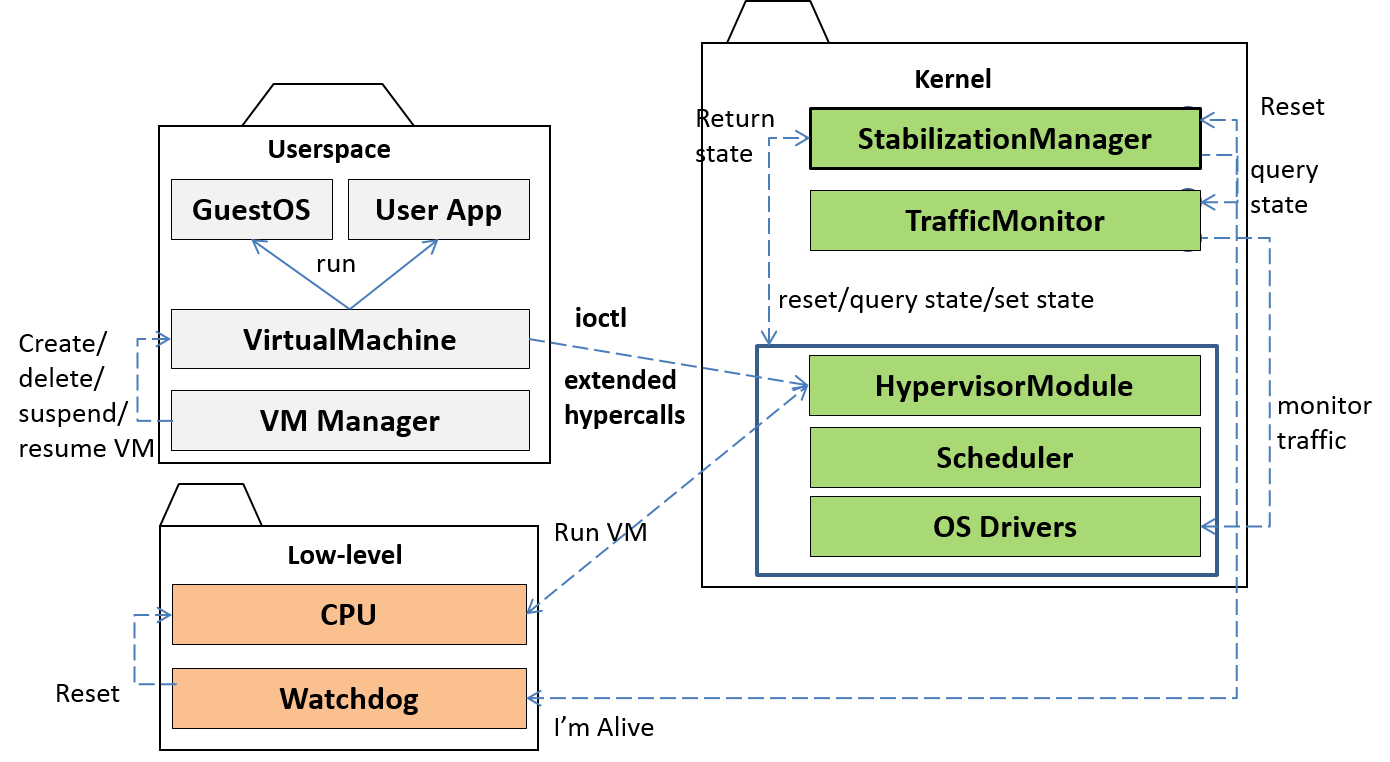
\includegraphics[width=12cm]{pictures/overview}
\par\end{centering}

\caption{\label{fig:The-overview-figure}The components of the self-stabilizing
hypervisor}
\end{figure}



\subsection{Security Model }

Our architecture is designed to provide defense against the following
threats/failures that hit the cloud infrastructures. 


\paragraph{VM State corruption. }

For example, a rootkit modifies the internal structures of a guest
OS, preparing to expand the attack surface into the hypervisor as
in \cite{Wang:rootkits:2009}. At every execution phase the SM checks
whether the state of every VM is changed comparing to the current
state. To accomplish the task the SM accesses VM internal structures,
being a part of the hypervisor. 


\paragraph{Malicious/corrupt inter-VM communication. }

A typical example is a VM guest sending malware to another one as
in \cite{Srivastava:2008:TAB:1433006.1433011}; the malware attacks
the target host, breaching the hypervisor defense. The defense can
be provided by inspecting the traffic between VMs. 


\paragraph{Greedy VM Allocation. }

There are a lot of legal ways for users to get more service from a
hypervisor than it is needed thus starving the latter. For example,
a guest sending many short requests including sensitive instructions
like CPUID causes context switches at the hypervisor; in a short time
the latter denies the service to other guests as in \cite{ddos-cpuid}.
The defense can be provided by monitoring all sensitive but not privileged
requests (like CPUID, RDTSC).


\subsection{The detailed description }

To illustrate the details of the self-stabilizing hypervisor architecture
we use UML class and state diagrams. In certain cases methods are
invoked in a system-specific manner (e.g. a system call, an asynchronous
call, an interrupt handler). We use the following UML stereotypes
to illustrate these specifics:
\begin{itemize}
\item \textbf{<\textcompwordmark{}<int>\textcompwordmark{}>} stands for
the method serving as an interrupt handler. 
\item \textbf{<\textcompwordmark{}<syscall>\textcompwordmark{}>} stands
for a system call. 
\item \textbf{<\textcompwordmark{}<async>\textcompwordmark{}>} stands for
an asynchronous method invocation. 
\end{itemize}
The following subsections provide the detailed description for all
the packages included into the architecture.


\subsubsection{Userspace}

The virtual machine manager is represented by the class \textit{VMManager}.
It creates and deletes virtual machines through its methods \textit{createVM}
and \textit{deleteVM}. At the user level, VMs are represented by the
class \textit{VirtualMachine}. When creating a VM, a user submits
the guest OS image and the initial configuration (e.g., the sizes
of its disk and memory spaces) of the VM being created. The guest
OS executes user applications.

Upon a VM creation request, the hypervisor driver receives the \textit{CREATE}
control system call and returns in response the ID of the newly created
VM (\textit{VMID}). For a newly created VM, a new thread (represented
by the class \textit{VMThread}) is launched. This thread sends RUN
messages to the hypervisor, addressing the related VM through its
VMID. The VM Manager may suspend/resume VMs at a request from a third
party (e.g., for performing quarantine or for billing purposes). Figure
\ref{fig:User-level-collaborations} illustrates the user-level collaborations. 

\begin{figure}
\begin{centering}
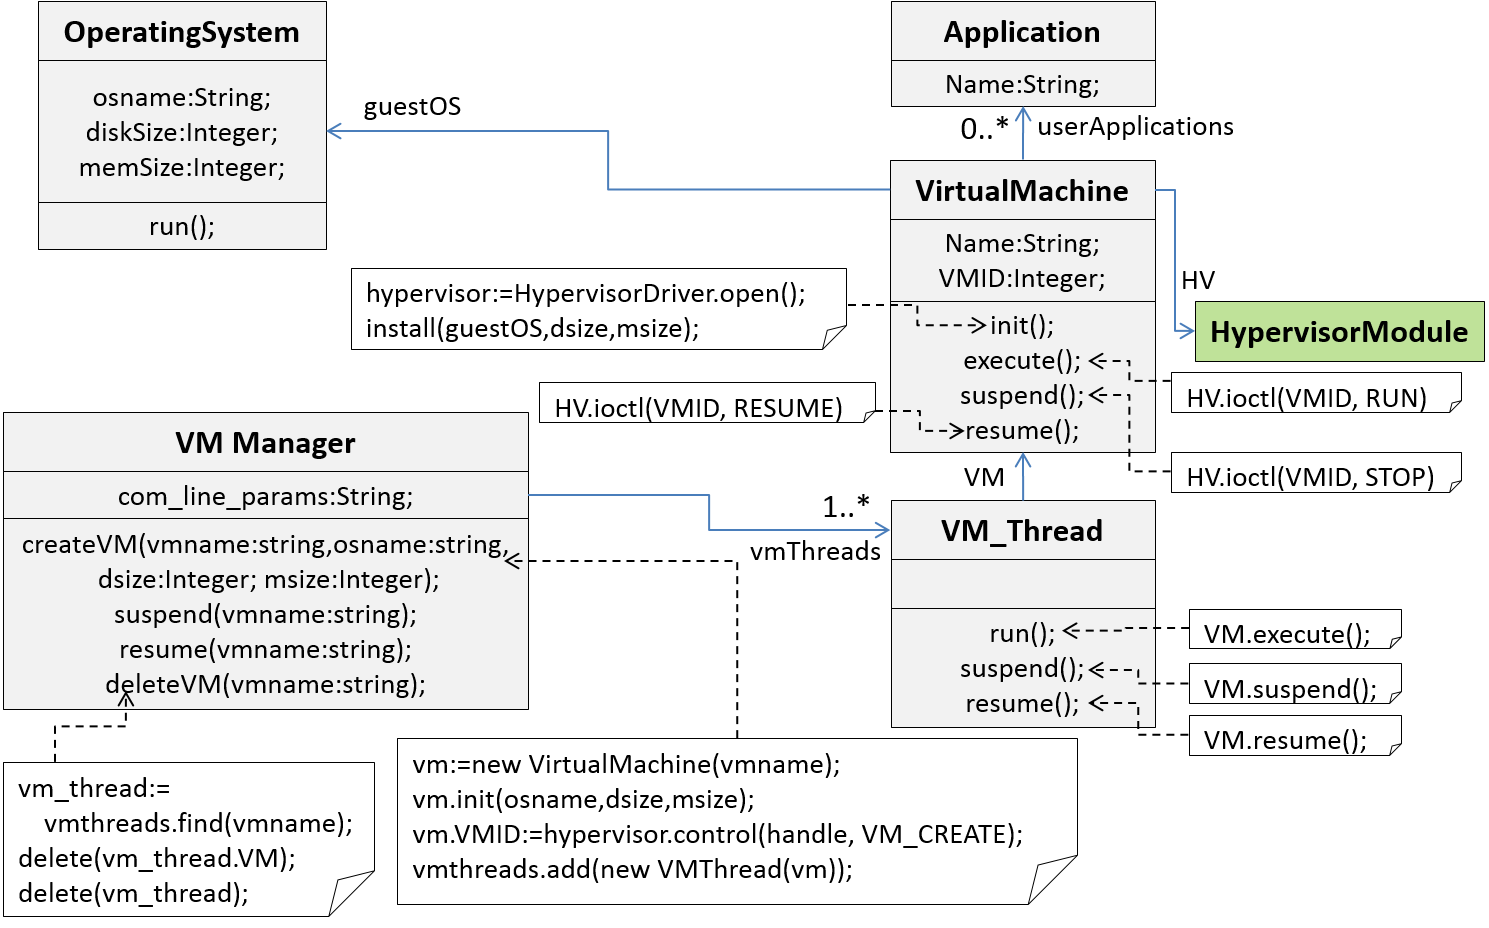
\includegraphics[width=12cm]{pictures/user-level}
\par\end{centering}

\caption{\label{fig:User-level-collaborations}User-level collaborations in
our architecture}
\end{figure}



\subsubsection{\label{sub:Hardware}Hardware}

This part represents the hardware abstraction of the architecture:
the system integrity checker and the CPU. The integrity checker (represented
by the class \textit{IntegrityChecker}) is characterized by the \textit{fire
period} (the time period in which the hardware triggers the integrity
checker code). If the integrity checker reveals modifications in the
OS code, the entire system is reset (through a reboot); otherwise
the reset task of detecting modifications is delegated to the watchdog.

The integrity checker resides in the memory that is write-protected
using hardware means. For example, in the Intel architecture this
is the memory associated with the System Management Mode (SMM) {[}2{]}.
This memory can be accessed only by the BIOS itself. TrustZone \cite{trust-zone}
provides the same features in the ARM architecture. We are working
on Intel computers and therefore use the SMM memory.

The OS kernel cannot tamper with the code we inject, thus unless an
attacker hacks/changes the SMM code, even on reboot, the Integrity
Checker code cannot be changed by any application besides the BIOS
itself. Because the kernel boot process typically runs before a malicious
party gains control, the SMM region remains unreachable for adversaries.
The SMM code is launched upon arrival of a hardware timer interrupt
(System Management Interrupt, shortly SMI) which arrives through an
out-of-band channel that is not governed by the kernel. A context
switch typically precedes the trusted code execution. Since a SMI
is generated by a hardware device and its behavior cannot be changed
a hacker gaining control over the system cannot change the SMM or
configure the hardware device that triggers the SMI. It should be
noted that the above mentioned context switch saves the full CPU status,
freezing kernel execution until the trusted code ends. Therefore checking
the integrity of the whole system is highly inefficient. One of improvements
suggested by us is to let the Integrity Checker verify that only the
watchdog is not modified. The watchdog, in turn, asynchronously verifies
the integrity of the entire system. Figure \ref{fig:The-hardware-layer}
describes the hardware layer. 

\begin{figure}
\begin{centering}
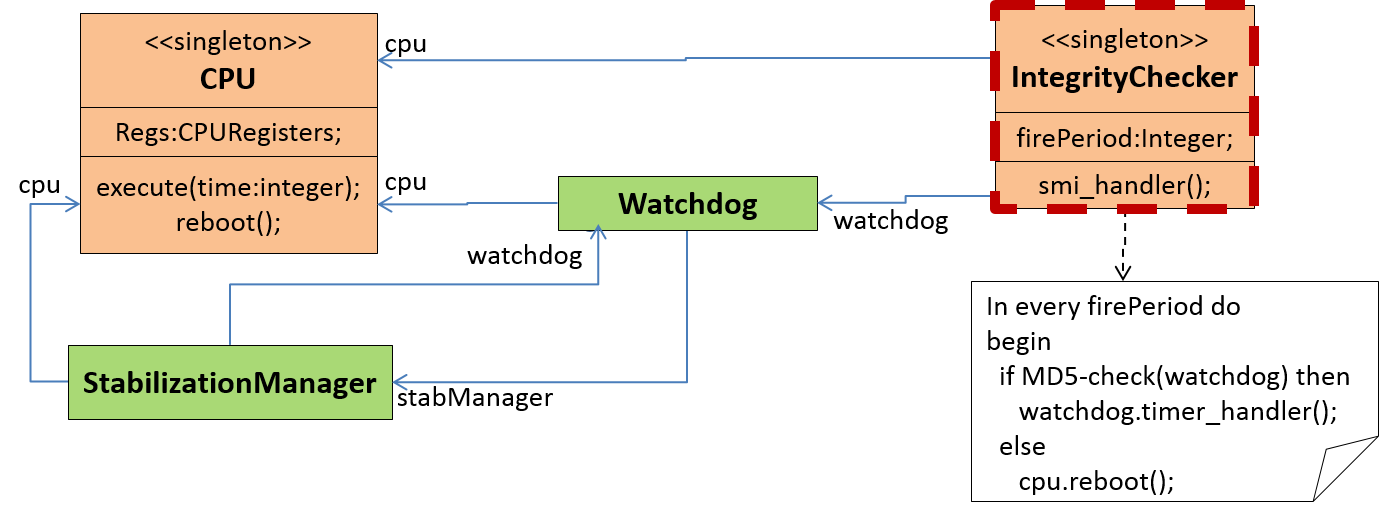
\includegraphics[width=12cm]{pictures/hardware}
\par\end{centering}

\caption{\label{fig:The-hardware-layer}The hardware layer}
\end{figure}



\subsubsection{Kernel}


\paragraph{Stabilizable components}

This subsection enumerates the architecture components whose states
is crucial for proper functioning of the hypervisor. The goal of the
stabilization manager is to make sure these states are stable. That
is why these components are referred to as the \textit{stabilizable
components}. They include:
\begin{itemize}
\item The hypervisor is represented by the class \textit{HypervisorModule}.
It possesses three (necessary) callbacks for the corresponding system
calls: opening, closing a device and getting control messages. 
\item The system scheduler is represented by the class \textit{Scheduler}.
It executes all processes/threads in the system, including those which
manage VM execution. The scheduler holds the collection of the objects
of the class \textit{VMThread} representing these threads. 
\item The components related to the system traffic are: I/O drivers and
the Traffic Monitor (the class \textit{TrafficMonitor}). The latter
monitors the traffic at the system I/O drivers.
\end{itemize}
The self-stabilization functionality is encapsulated in the Stabilization
Manager (SM) that is described by the class StabilizationManager.
The SM checks and, if needed, enforces the system stability in every
predefined time period; the corresponding actions are done within
the timer interrupt handler \textit{timer\_handler}. Stabilizable
components are provided in Fig. \ref{fig:The-stabilizable-components}. 

\begin{figure}
\begin{centering}
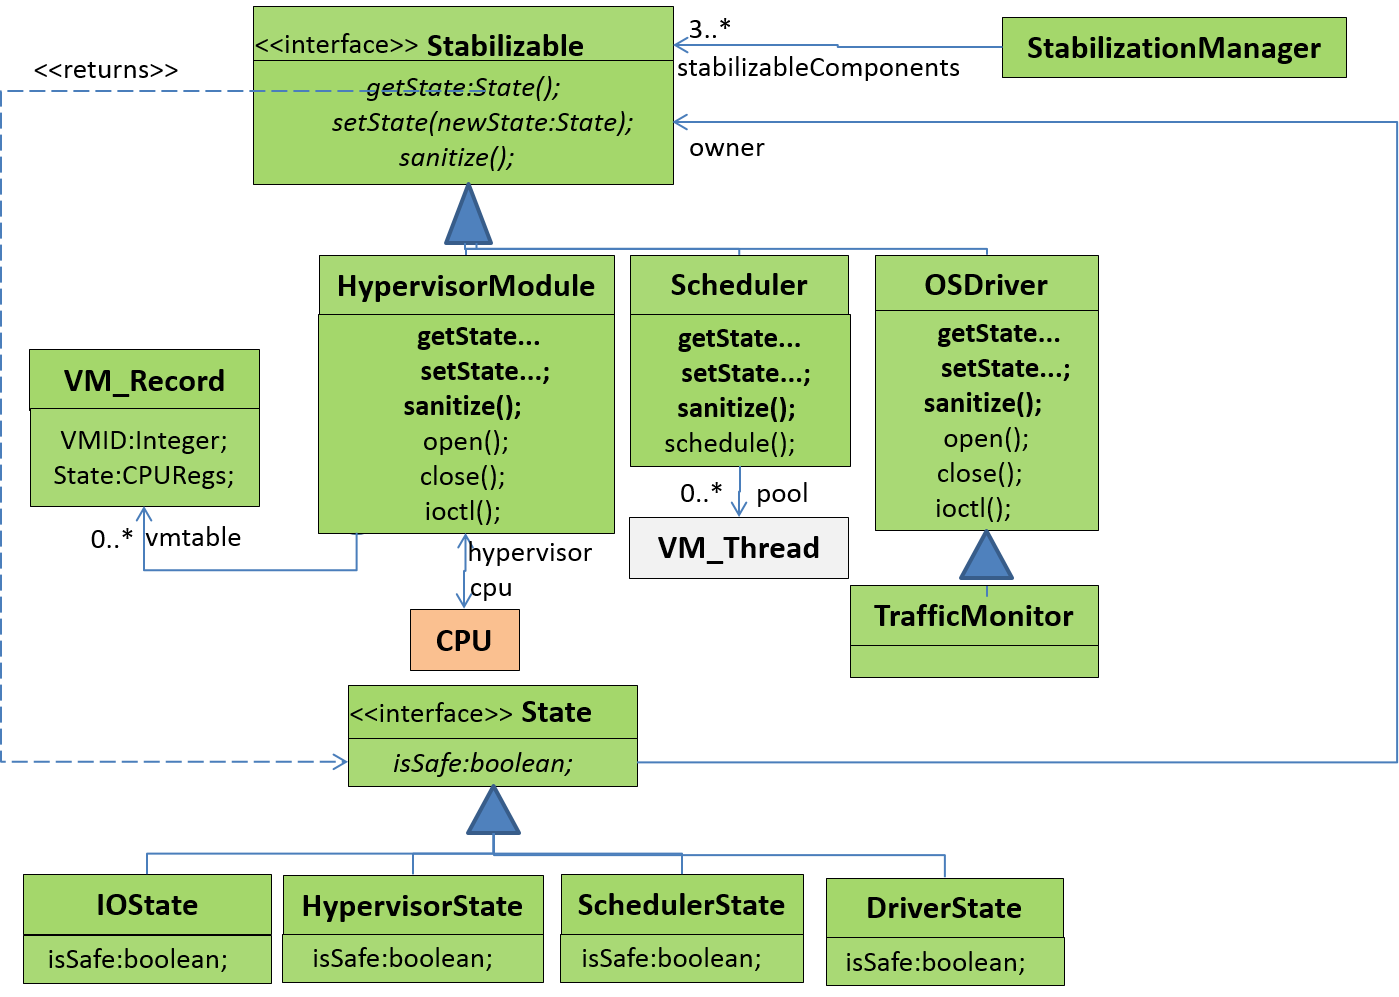
\includegraphics[width=12cm]{pictures/stabilizable-components}
\par\end{centering}

\caption{\label{fig:The-stabilizable-components}The stabilizable components}
\end{figure}



\paragraph{Bringing the system into a stable state }

In order to collaborate with the SM the stabilizable components possess
the following capabilities: \textit{get state}, \textit{set state}
and \textit{sanitization}. When checking the system state the SM gets
states from every stabilizable component within the system; if needed
the new (stable) state is set. Sanitization action cleans the traits
of the previous activities (e.g., flushing buffers). A state of every
stabilizable component is represented by the class \textsf{State}
and its subclasses. Every such subclass represents the state of a
concrete stabilizable component and (by virtue of owning the \textsf{isSafe}
method) is capable of determining whether it is stable. 

The actions for verification and enforcement of system state stability
represent defenses against various attacks (e.g., DOS attack, rootkit
activity). Defenses may be state-based (i.e., do not kill the VM issuing
DOS attacks during several timer iterations; kill it afterwards).
We specify these defenses using the language based on guarded commands,
see Section \ref{sub:The-attack-scenarios} for more details. Guarded
commands are chosen because they are a natural way to express state-based
actions as in \cite{Dolev:2009:SPC:1552309.1552312}. 

There are sophisticated actions for inteligent system reset (referred
to as \textit{soft reset}); for example, suspend or kill only malfunctioning
VMs instead of rebooting the computer. If no soft reset actions ar
available in a given situation then the computer is rebooted (\textit{hard
reset}). Once in a predefined period the recent stable state is saved
in the storage (represented by the class \textit{StatesStorage}) and
can be used to recover the recent stable state during the soft reset.

The watchdog (represented by the class \textit{Watchdog}) is characterized
by the \textit{kick period}, i.e., the time period during which at
least one \textit{I\_Am\_Alive} message should arrive. \textit{I\textquoteright{}m
Alive} messages are sent by the SM invoking the\textit{ i\_am\_alive}
method; this happens after ensuring that the system state is stable.
\textit{I\_Am\_Alive} messages causes the watchdog timer to be postponed.
The watchdog timer fires an interrupt when \textit{I\_Am\_Alive} messages
do not arrive during a while. The watchdog searches for a reset strategies;
soft reset actions are executed if supported, otherwise the computer
is rebooted. 

It should be noted that bringing the system into a stable state is
too time-consuming for a task executed within an interrupt handler
so the SM collects and sets individual states in the asynchronous
manner. 

\begin{figure}
\begin{centering}
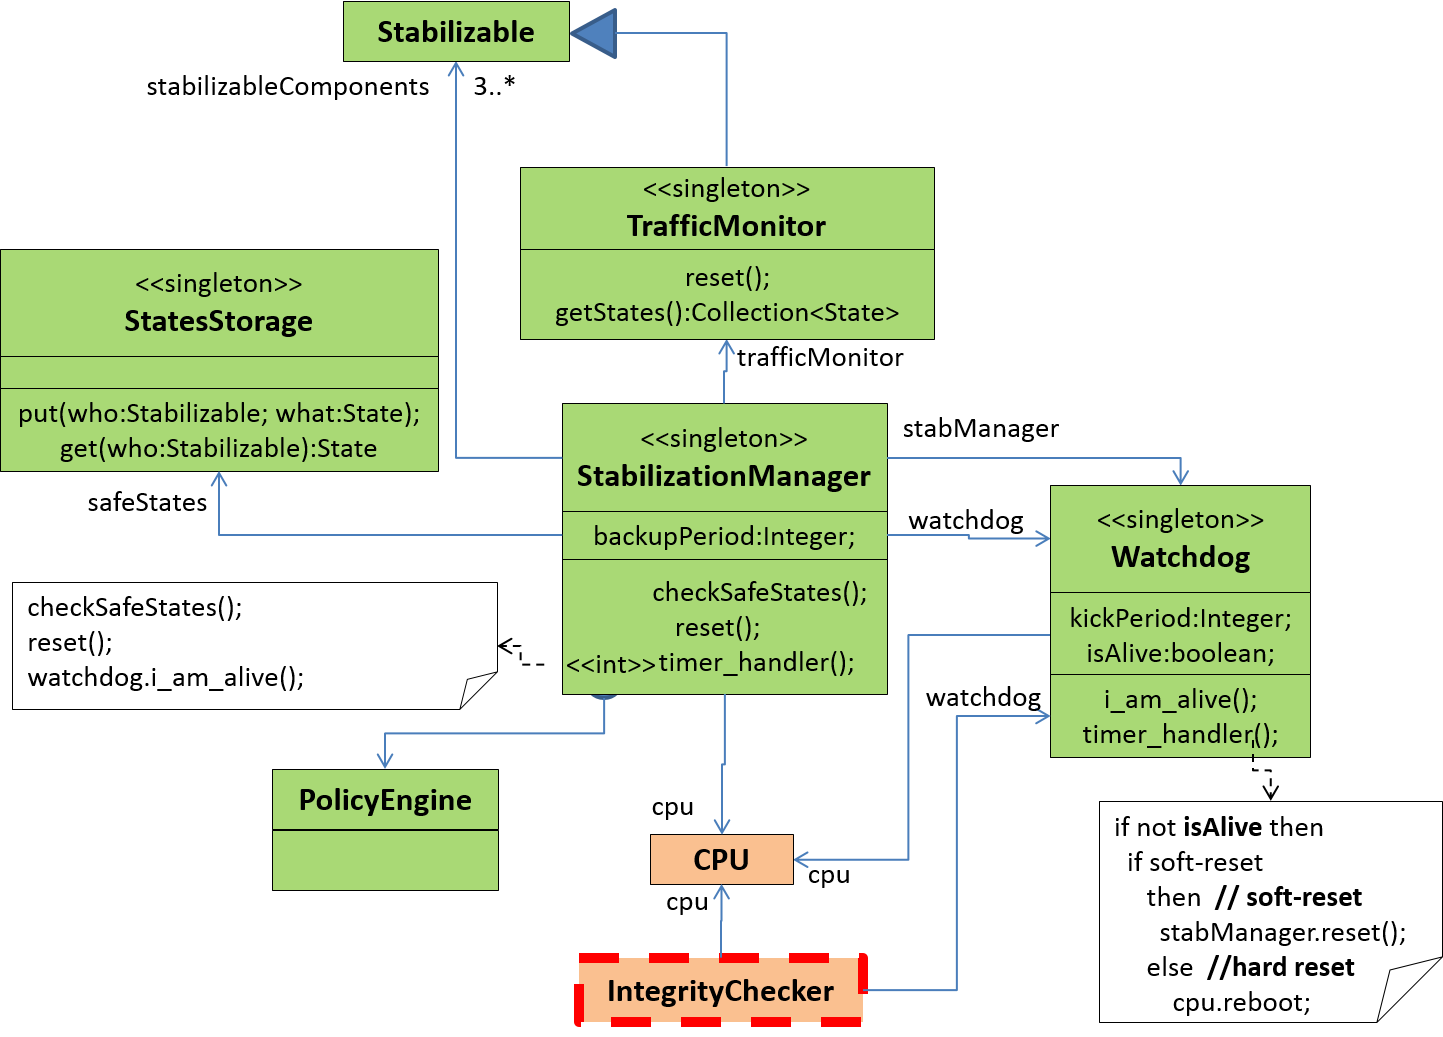
\includegraphics[width=12cm]{pictures/kernel-collabs}
\par\end{centering}

\caption{\label{fig:The-kernel-level-collabs}The kernel level collaborations}
\end{figure}


The entire life cycle of the Stabilization Manager is summarized in
Fig. \ref{fig:The-entire-self-stabilization-logic} using three state
machines. The following denotations do not constitute a part of the
recent UML standard \cite{uml-spec} and explained below: 
\begin{itemize}
\item The Integrity Checker is wrapped by the thick red dashed line; showing
that we put it into the hardware-protected memory zone. 
\item The History pseudonode serves either as the target node (as in the
UML standard, denoting the current execution context) or as the source
node (denoting an arbitrary state in a given state machine). In summary
the usage of the History node illustrates that a timer interrupt causes
the execution leave the current context at any possible state. 
\item State transition priority. The stereotype \textbf{<\textcompwordmark{}<high-priority>\textcompwordmark{}>}
near the interrupt transition means that the latter occurs as soon
as possible. 
\end{itemize}
\textcolor{black}{To check whether the system state is stable, the
Stabilization manager uses the following sources of information:}
\begin{itemize}
\item \textcolor{black}{System logs. For example rootkits send sensitive
information through the network, causing periodic traffic bursts.
System logs can help detect rootkits with quite sophisticated scenarios.
However, an adversary might modify system logs.}
\item \textcolor{black}{Looking after system model changes. A system model
represents security-related structures typically altered by rootkits
(e.g., process table, driver jump table). Without relying on (possibly
damaged) system logs, the SM checks whether these structures underwent
changes.}
\end{itemize}
The Stabilization Manager brings a system in a consistent state as
part of a periodic consistency checks following a timer interrupt.
If a guarded command running in the SM context detects severe problems
(e.g., inconsistencies in the system scheduler), then the system reset
may be fired immediately. For example, a rootkit trying to inject
code into the kernel code area (usually write-protected) triggers
a protection fault. The latter is intercepted, triggering immediate
system reset. 

\begin{figure}
\begin{centering}
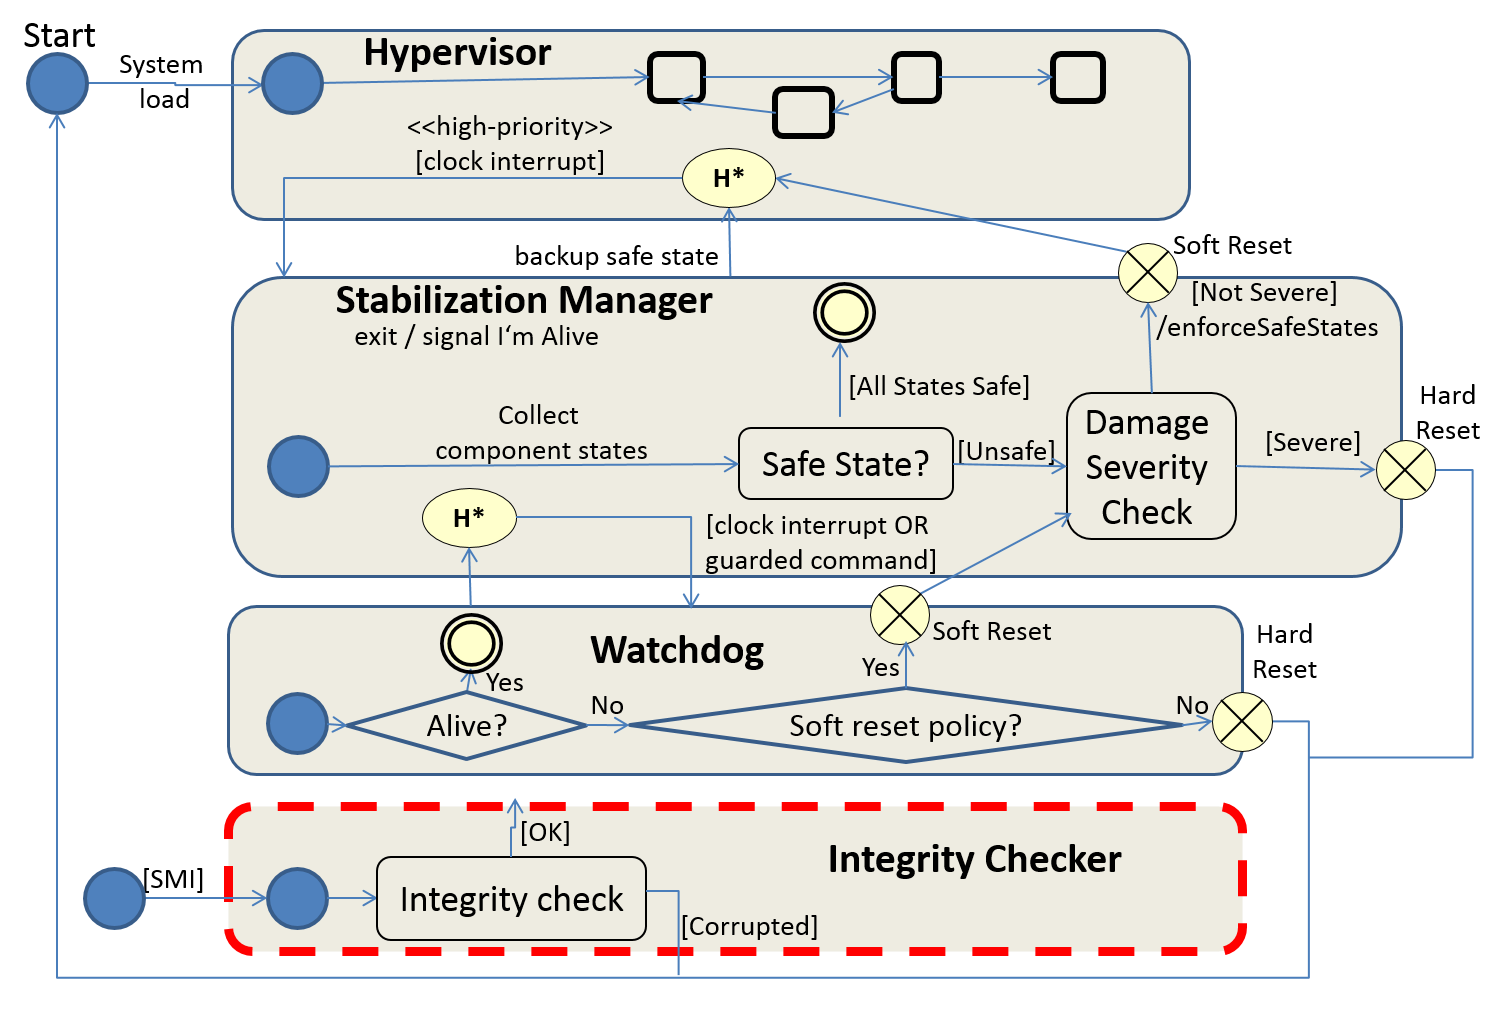
\includegraphics[width=12cm]{pictures/state-machine-selfstab}
\par\end{centering}

\caption{\label{fig:The-entire-self-stabilization-logic}The entire self-stabilization
process summarized }
\end{figure}




\section{\label{sec:The-prototype}The proof of concept}


\subsection{\label{sub:The-attack-scenarios}The attack scenarios modeled in
the prototype}

Our prototype implements two scenarios that illustrate particular
cases of attacks against hypervisors: denial of service and rootkit
activities. In both scenarios defense policies are expressed in the
terms of guarded commands \cite{Dijkstra:1975:Guarded}. Following
\cite{Dolev:2009:SPC:1552309.1552312} guarded commands are a natural
way to express state-based actions. 


\paragraph{Denial Of Service (DOS) }

In general we distinguish between two kinds of denial of service attacks:
\begin{itemize}
\item Local. A VM sends a lot of sensitive requests (e.g. CPUID \url{http://en.wikipedia.org/wiki/CPUID})
to the hypervisor. Handling sensitive (but not provileged) instructions
hypervisors (in particular KVM) gains the execution context, handles
these instructions and passes the control back to the sending VM.
Such context switches starve hypervisor out of computational resources,
see \cite{ddos-cpuid} for more details.
\item Network-based. A VM floods the network with requests starving the
TCP-related resources.
\end{itemize}
At the hypervisor level, our system handles DOS attacks as follows:
at every SM iteration we count the number $NR$ of DOS requests. If
$NR$ exceeds the certain threshold $Threshold$ we suspice a VM to
run an attacker. If $NR$ remains above $Threshold$ during several
SM iterations, we conclude that a DOS attacker continues to operate
and kill the VM running an attacker. If $NR$ becomes very high, exceeding
the threshold $MaxThreshold$ (which is significantly bigger than
$Threshold$) we kill the VM executing an attacker immediately.


\paragraph{Rootkit activities}

Our system detects attempts to modify the contents of the Interrupt
Description Table (IDT) that contains the entries to software interrupt
handlers (also to system calls because a system call is a particular
case of software interrupt). If a party running at some VM tries to
modify the IDT of the corresponding virtual CPU we assume that this
party is malicious and kill the corresponding VM. This is because
hooking the system control flow (in particular interrupt handlers)
is the preparatory stage towards breaching into the hypervisor as
in \cite{intel-systret,defense-rootkit-attacks,Wang:rootkits:2009}.

The guarded commands for handling IDT changes are provided below:

\begin{multline*}
\forall VMID\in VirtualMachineIDs\cdot\\
IDT\_Changed(VMID)\wedge VM\_Rebooted(VMID)\mapsto KillVM(VMID);
\end{multline*}


and for handling of DOS requests: 

\begin{multline*}
\forall VMID\in VirtualMachineIDs\cdot\\
NumOfRequests(VMID,NR)\rightarrow true;\\
NR>Threshold\rightarrow NumOfAttackingIterations(NA);\\
NA>MaxAttackingIterations\rightarrow KillVM(VMID);\\
NA<MaxAttackingIterations\wedge NR>MaxReqThreshold\rightarrow KillVM(VMID)
\end{multline*}


Figure \ref{fig:The-defense-state-machines} provides the state machines
that illustrate both defense policies.

\begin{figure}
\begin{centering}
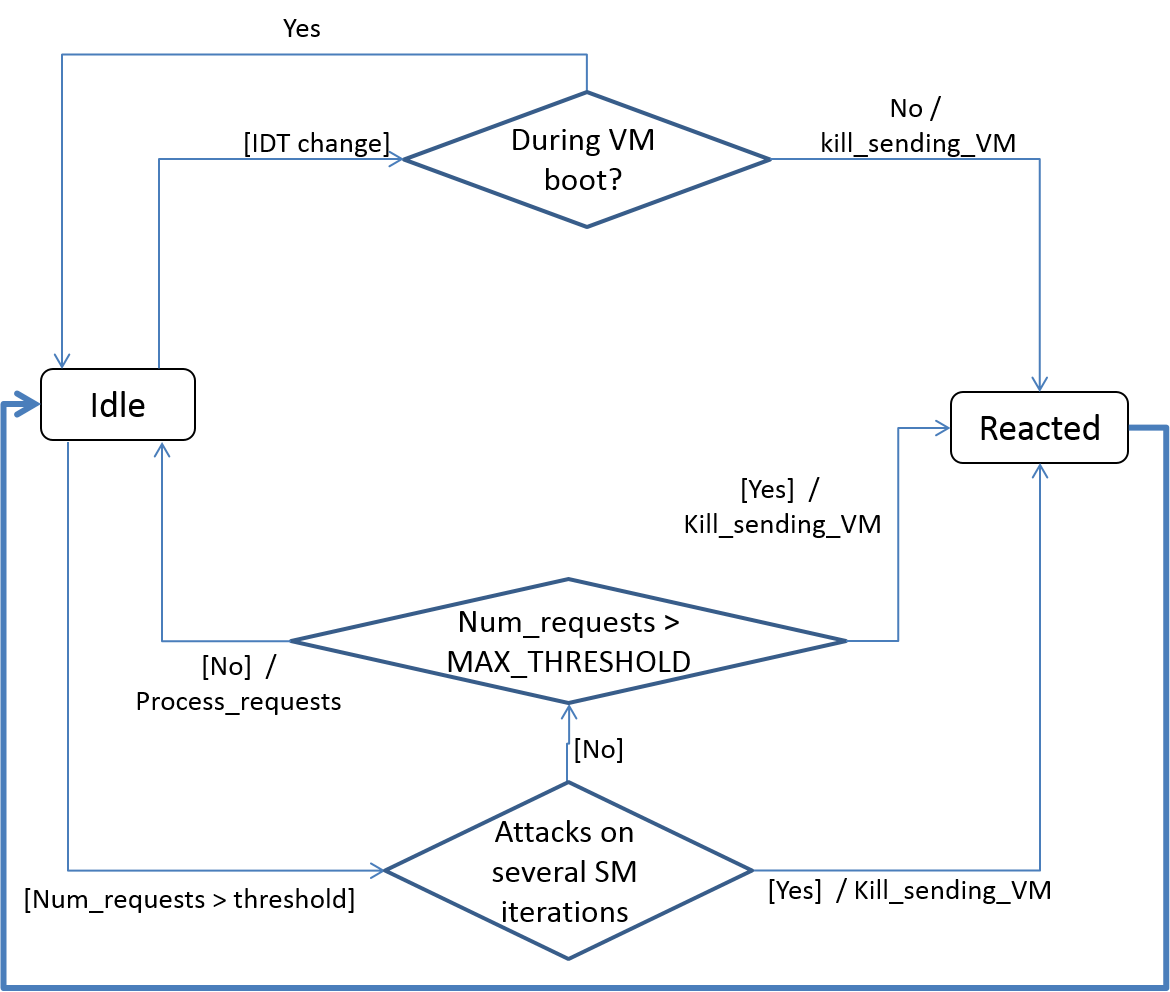
\includegraphics[width=12cm]{pictures/defense-sms}
\par\end{centering}

\caption{\label{fig:The-defense-state-machines}The state machines for the
defense policies implemented in our ptototype}
\end{figure}



\subsection{\label{sub:Implementation-Issues}Implementation Issues}

We are implementing the prototype as a Linux kernel module. Its current
version has the following timer interrupt handlers installed: The
SM timer and the watchdog timer. The SM timer handler does the following:
\begin{itemize}
\item In every execution it checks whether the system state is stable and
in case of need brings the system into a stable state. After these
actions are finished the watchdog timer signal is postponed, thus
illustrating the I'm Alive message.

\begin{itemize}
\item The system state is assumed to be stable if no IDT modifications and
no DDOS attacks are noticed.
\item If the system state is unstable then the SM brings it to a stabe state
as it is described in the previous section , ``The attack scenarios''.
\end{itemize}
\item Once in several executions of the SM timer handler the system state.


The watchdog timer reboots the OS, issuing the Linux system call .

\end{itemize}
We have implemented the first version of the Traffic Monitor. It intercepts
the network traffic between guests, printing out short statistics
about it (e.g., number of bytes). This is done by finding the handlers
for the TCP system calls (i.e., \textsf{sendv}, \textsf{recv}) in
the system call table, following the approach of \cite[Section 7]{pfoh-vmmonitor-2013}.
To make a full-fledged traffic sensor we still have to treat special
cases like the presence of VirtIO infrastructure \cite{VirtIO-Russell}
that consists of special drivers processing I/O at the guest side. 

We are running our prototype on an Intel architecture so we are using
the memory associated with System Management mode (SMM, \cite{GMU-CS-TR-Evasion-2011-8})
to provide the hardware-based write-protection of the Integrity Checker
code. Most of the modern hardware support hardware-based memory protection.
The integrity checker code runs in SMM and is triggered by the hardware
timer. Such a signal is guaranteed to arrive regardless of software
behavior. 

\textcolor{black}{It should be noted that in order to detect rootkits
the whole OS kernel (not just the Stabilization Manager) should be
checked for changes. The inefficiency of this operation is aggravated
by the fact that the Integrity Checker runs it synchronously, freezing
the whole OS. We suggest the following improvement that is supposed
to make the stabilization check more efficient:}
\begin{itemize}
\item \textcolor{black}{Let the Integrity Checker verify the integrity of
the Watchdog solely because the Watchdog module is relatively small.}
\item \textcolor{black}{The Watchdog modulevafter its integrity is confirmed,
launches an asynchronous system state check. }
\end{itemize}
\textcolor{black}{In order to minimize delays caused by the SMM code
execution, extensive system state checks may be carried out at night
time.}



\section{\label{sec:Related-Work}Related Work}



\section{\label{sec:Conclusions-and-Future-Work}Conclusions and Future Work}

In this work we have suggested a novel self-stabilizing hypervisor
architecture which is capable of performing a wide range of stabilizing
actions starting from coarse-grained ones (like killing suspicious
VMs) to fine-grained ones (e.g., stopping guest applications whose
behavior seems to be suspicious). We have provided the conceptual
description of the architecture as well as the formal proof of its
self-stabilization. As a proof of concept we implement the self-stabilization
functionality in the KVM hypervisor \cite{kvm-site}. The design proposed
in this report adds the self-stabilization feature to the common hypervisor
architecture. We have also reviewed existing industrial products related
to the hypervisor level as a first step towards extending the current
work from a local node to a full distributed cloud setting. Finally,
we note that our implementation was tested with several initial denial
of service and rootkits attacks and exhibit low overhead in consistency
monitoring and guarded commands execution for recovering the system
to regain consistency. We plan to carry out more extensive experiments
using known test workloads like the rootkit repositories mentioned
in \cite{Wang:rootkits:2009} and to collect results.

Several future research directions we propose are provided below: 
\begin{itemize}
\item Executing guarded commands in a stabilization-preserving way. So far
our prototype has several defense policies (Denial of Service (DOS)
and rootkit defenses) hardcoded. We intend to support user-defined
specifications of defense policies. We intend also to build a compiler
that will transform our specifications into the behaviorally equivalent
set of actions while preserving stabilization.
\item Specifying device drivers formally. Our architecture is a part of
the Linux system and thus is not object-oriented. To bridge the gap
between the conceptions of our architecture (which is not object-oriented)
and UML (which describes object-oriented conceptions) we used stereotyping,
making specifications more informal. We intend to learn how to map
OS-related concepts into the OO domain following the literature (like
\cite{sertic-rus-rac:uml-realtime:2003}) and apply the approaches
to our specification thus making the latter more rigorous. 
\item Guests issuing DOS attacks. One of main challenges posed when detecting
DOS attacks is 'moving attackers', i.e. the party issuing DOS packets
(attacker) frequently changes the source IP. Source-based attacker
spotting is therefore complicated. Moving attacks in cloud infrastructures
can be easily mounted by placing attackers on migrating VMs (see \cite{key:article}
for further details on VM migration techniques). Making the Traffic
Monitor capable of recognizing various patterns (e.g., periodic bursts)
could improve the precision of DOS recognition. 
\item Comprehensive Security Model. The security model supported in our
architecture covers several common threats/failures plaguing cloud
infrastructures: VM state corruption, malicious inter-VM communication
and greedy resource allocation. We intend to study various security
models used in cloud infrastructures, create a comprehensive taxonomy
of VM threats and enhance our security model. \end{itemize}



\bibliographystyle{abbrv}
\bibliography{sample}
\end{abstract}

\end{document}
